\documentclass{article}
\usepackage[utf8]{inputenc}

\title{test1}
\author{hanspeter6 }
\date{November 2019}

\usepackage{natbib}
\usepackage{graphicx}

\begin{document}

\maketitle

\section{Introduction}
This is a 2013 review of ICA by \cite{hyvarinen2013independent} that considers developments in the field since 2000.

Main topics are:
\begin{itemize}
  \item Analysis of causal relations
  \item Testing independent components
  \item Analysing multiple data sets (three-way data)
  \item Modelling dependencies between the components
  \item Improved methods for estimating the basic model
\end{itemize}

OK LETS BEGIN....

\begin{figure}[h!]
\centering
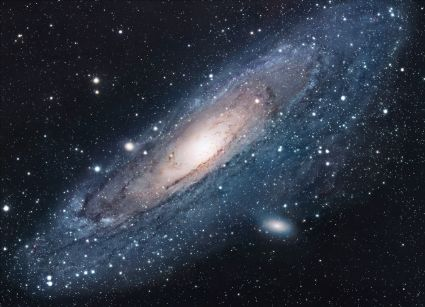
\includegraphics[scale=1.7]{universe}
\caption{The Universe}
\label{fig:universe}
\end{figure}

\section{Conclusion}
``I always thought something was fundamentally wrong with the universe'' \citep{adams1995hitchhiker}

\bibliographystyle{apalike}
\bibliography{references}
\end{document}
